\documentclass[border=1mm]{standalone}

\usepackage{tikz}
\usepackage{pgf-umlcd}
\usetikzlibrary{positioning,fit,calc}
\usetikzlibrary{shapes.multipart}

\newsavebox\mybox

\begin{document}

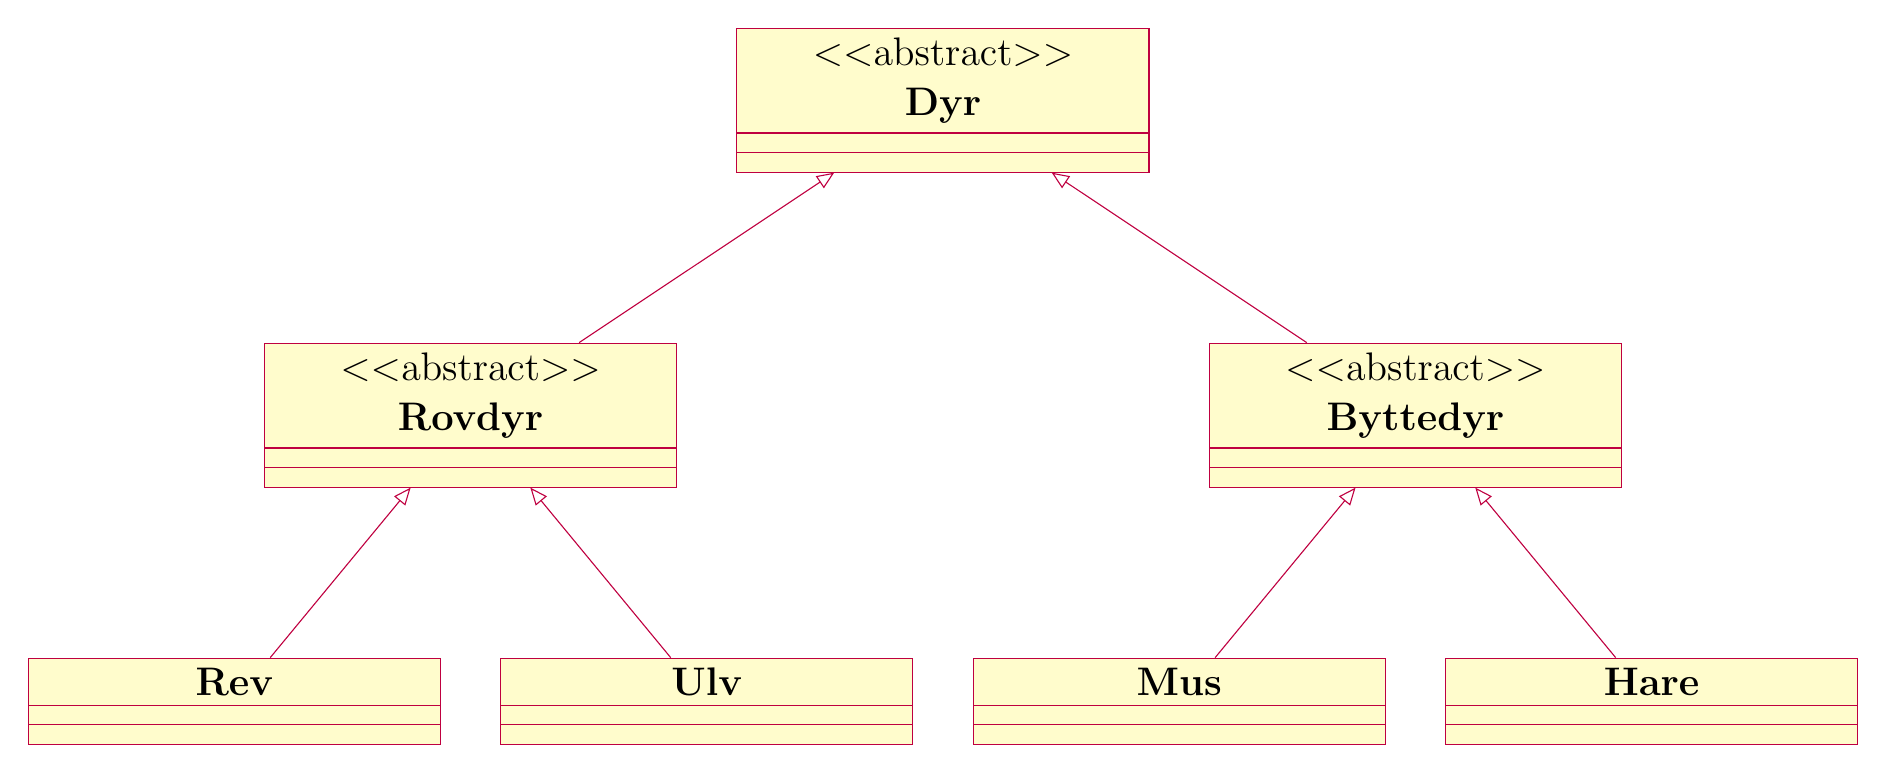
\begin{tikzpicture}
          \tikzstyle{every node}=[font=\Large]

      \begin{abstractclass}{Dyr}{0 , 0}
      \end{abstractclass}

      \begin{abstractclass}{Rovdyr}{-6 , -4}
	 \inherit{Dyr}
      \end{abstractclass}

      \begin{abstractclass}{Byttedyr}{6 , -4}
	 \inherit{Dyr}
      \end{abstractclass}

      \begin{class}{Rev}{-9 , -8}
	 \inherit{Rovdyr}
      \end{class}

      \begin{class}{Ulv}{-3 , -8}
	 \inherit{Rovdyr}
      \end{class}

      \begin{class}{Hare}{9, -8}
	 \inherit{Byttedyr}
      \end{class}

      \begin{class}{Mus}{3 , -8}
	 \inherit{Byttedyr}
      \end{class}

\end{tikzpicture}

\end{document}

       \tikzstyle{every node}=[font=\footnotesize]
